\documentclass[11pt,a4paper]{article}
\usepackage[margin=2cm]{geometry}
\usepackage{amsmath,amssymb}
\usepackage{booktabs,float,graphicx,enumitem,tabularx}
\usepackage[table]{xcolor}
\usepackage{tikz}
\usetikzlibrary{arrows.meta,positioning,fit,backgrounds}
\usepackage{listings}
\usepackage[T1]{fontenc}
\usepackage{lmodern}
\usepackage{microtype}
\usepackage[hidelinks]{hyperref}
\lstset{basicstyle=\ttfamily\scriptsize,breaklines=true,columns=fullflexible,frame=single,keepspaces=true}
\setlength{\parindent}{0pt}
\setlength{\parskip}{4pt}
\newcommand{\studentname}{Erik Mirzoyan}
\newcommand{\repourl}{https://github.com/10mirzoyan71/photonicsai-lab}

\begin{document}
\begin{center}
{\Large\bfseries PhotonicsAI --- AI-Driven Science and Autonomous Laboratories}\\[3pt]
{\large Homeworks 4 and 5: the PhotonicsAI Lab Assistant}\\[6pt]
Name: \studentname\\[2pt]
Code: \url{\repourl}
\end{center}

\textbf{What it is.} Homeworks 1--3 built three agent systems: physics-informed modelling of the Silverbox oscillator
(HW1), human-in-the-loop focusing of light through a scattering medium on a simulated bench (HW2), and an agent that
drives a real lab camera through MCP (HW3). This project puts them under one roof as a \textbf{laboratory with a director
and teams}, and makes it a web application: a person asks the lab a question in plain words, approves steps on the real
camera with a button, does what needs hands (blocking the light), and watches the camera, the team reports and the
results while the agents work. The new parts are:
\begin{itemize}[leftmargin=*,itemsep=1pt]
\item \textbf{two more levels of hierarchy}: a director above the three homework systems, which now work as teams;
\item \textbf{questions passed up the hierarchy}: a team's question to the person reaches the person through the director,
  also when the process is restarted between the question and the answer;
\item \textbf{a web application} (Streamlit) with approval and action cards, a camera panel, verified results, a token
  meter, a replay mode, and runs that can be continued or retried;
\item \textbf{four new instrument tools} (black level, ADC bit depth, temperature, TIFF export; Homework~3, section~(g)),
  which the instrument team uses on its own;
\item \textbf{a token budget}: every model call is counted, and the design keeps a run to about 1\,\% of the weekly
  usage limit of a Claude subscription.
\end{itemize}

%======================================================================
\section*{1. The hierarchy}
%======================================================================
\begin{figure}[H]\centering
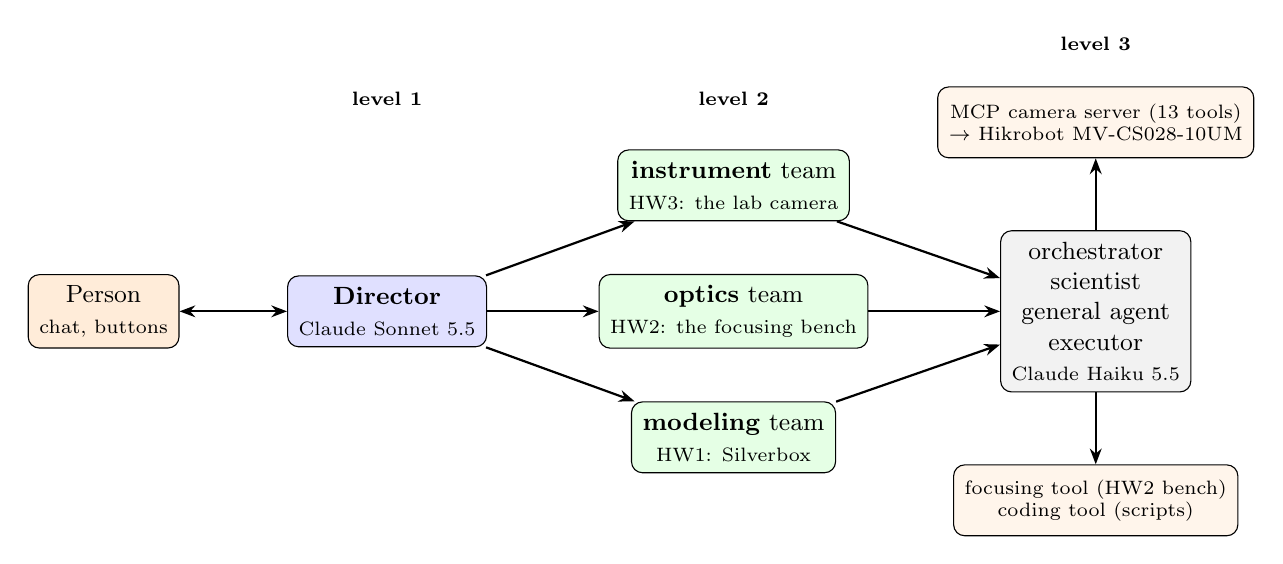
\begin{tikzpicture}[font=\small, b/.style={draw,rounded corners,align=center,inner sep=4pt,minimum height=9mm},
  a/.style={-{Stealth[length=2mm]},thick}]
\node[b,fill=orange!15] (p) at (0,0) {Person\\\scriptsize chat, buttons};
\node[b,fill=blue!12] (d) at (3.6,0) {\textbf{Director}\\\scriptsize Claude Sonnet 5.5};
\node[b,fill=green!10] (i) at (8,1.6) {\textbf{instrument} team\\\scriptsize HW3: the lab camera};
\node[b,fill=green!10] (o) at (8,0) {\textbf{optics} team\\\scriptsize HW2: the focusing bench};
\node[b,fill=green!10] (m) at (8,-1.6) {\textbf{modeling} team\\\scriptsize HW1: Silverbox};
\node[b,fill=gray!10] (s) at (12.6,0) {orchestrator\\scientist\\general agent\\executor\\\scriptsize Claude Haiku 5.5};
\node[b,fill=orange!8,font=\scriptsize] (t1) at (12.6,2.4) {MCP camera server (13 tools)\\$\to$ Hikrobot MV-CS028-10UM};
\node[b,fill=orange!8,font=\scriptsize] (t2) at (12.6,-2.4) {focusing tool (HW2 bench)\\coding tool (scripts)};
\draw[a,{Stealth[length=2mm]}-{Stealth[length=2mm]}] (p) -- (d);
\draw[a] (d) -- (i); \draw[a] (d) -- (o); \draw[a] (d) -- (m);
\draw[a] (i) -- (s); \draw[a] (o) -- (s); \draw[a] (m) -- (s);
\draw[a] (s) -- (t1); \draw[a] (s) -- (t2);
\node[font=\scriptsize\bfseries] at (3.6,2.7) {level 1}; \node[font=\scriptsize\bfseries] at (8,2.7) {level 2};
\node[font=\scriptsize\bfseries] at (12.6,3.4) {level 3};
\end{tikzpicture}
\caption{The three levels. The person talks only to the director; each team is the agent graph of Homeworks 1--3
with its own tools; the specialists inside a team call the tools.}
\end{figure}

\begin{center}\small
\begin{tabularx}{\linewidth}{@{}lXl@{}}
\toprule
level & role & budget\\ \midrule
1 director & splits the request into team tasks, passes VERIFIED numbers from one team to the next, stops for the
  person before a task changes the real camera, writes the final report from VERIFIED records only & 6 decisions\\
2 teams & \textbf{instrument}: the lab camera behind the HW3 MCP server (exposure, gain, ROI, black level, ADC bit
  depth, temperature, captures, time series, frame analysis, TIFF) and a coding tool; \textbf{optics}: the simulated
  HW2 bench with the focusing tool, whose camera model can take measured numbers; \textbf{modeling}: the HW1 Silverbox
  record, the identified Duffing equation and the kept network, with a coding tool &
  8 / 6 / 6 decisions\\
3 specialists & orchestrator (decides), scientist (theory and plan), general agent (critique), executor (the only one
  with tools); inside the instrument team a hardware turn: decide $\to$ command $\to$ measure $\to$ decide &
  12 steps per hardware turn\\
\bottomrule
\end{tabularx}
\end{center}

%======================================================================
\section*{2. How the levels work together}
%======================================================================
\textbf{The director} is a LangGraph \texttt{StateGraph} with the nodes \texttt{director}, \texttt{human} and one node per
team, on a thread checkpointed in SQLite. Each decision is a structured output (\texttt{DirectorDecision}: the next team
or \emph{human} or \emph{finish}, a task, a question, why it stops, the pending step, a reason), so it can only name
teams that exist. A task must be self-contained: the team does not see the director's dialogue, so the director copies
into it every number it needs from earlier VERIFIED records (e.g.\ the measured read noise for the optics team). Code,
not the model, enforces the rules: \emph{finish} is refused while no team has returned a VERIFIED record; the person is
asked for approval only before an instrument-team task and at most once per run (a second request runs the task
directly); there is no approval stop before the final report; and after the budget the run stops with what it has.

\textbf{A team} is the Homework~3 agent graph built with the team's tools and prompts (\texttt{agent\_v3.build\_graph}).
It runs on its own checkpointed thread (\texttt{<run>-<k>-<team>}) and in a separate Python thread, so it is an
independent graph and not a subgraph of the director's node. Teams without hardware get a decision schema without the
hardware role, so their orchestrator cannot choose it. A team returns its last executor record that is VERIFIED (the
numbers a tool printed), and only these records go back to the director.

\textbf{A question from a team} (in a hardware turn: ``please block the light'') pauses the team's graph with an
interrupt. The director's team node then pauses the director with the same question, so the person answers everything
in one place; the answer resumes the team with \texttt{Command(resume=answer)}. After every resume LangGraph runs the
node again from the start and \texttt{interrupt()} returns the answers already given in order; the node therefore first
replays one interrupt per answer the team has already received and only then passes on the next question. Because both
levels are checkpointed, a paused run can be continued from a new process (a test restarts between the question and
the answer), and \emph{Retry} runs on from the last checkpoint after an error.

\textbf{The model backend} is the Claude Code CLI in print mode with its own tools switched off
(\texttt{claude -p -{}-output-format json -{}-tools "" -{}-json-schema ... -{}-effort low}), logged in with a Claude subscription,
so no API key is needed; the executor's tool calls come back as JSON and are run by the project's own tools. Any
LangChain chat model can be used instead (\texttt{make\_backend}).

%======================================================================
\section*{3. The web application}
%======================================================================
\texttt{python -m streamlit run lab/app.py} opens the app (\texttt{lab/app.py} draws the page; \texttt{lab/app\_core.py}
runs each run on a worker thread, so the page refreshes every second while the agents work, and lists the saved runs).
\begin{itemize}[leftmargin=*,itemsep=1pt]
\item \textbf{Chat}: the request, the director's decisions, each team's report with its VERIFIED record, and the team's
  internal work (orchestrator, scientist, executor, every camera command and its result) in a box per task.
\item \textbf{Approval card} (Approve / Refuse with a reason) and \textbf{action card} (Done, or an answer in words) in
  place of typed replies, so a typing slip cannot be read as a refusal (it happened in the first terminal run).
\item \textbf{Camera panel}: the newest frame the instrument team captured, with its exposure, gain and levels, and the
  last MCP call. \textbf{Verified results}: the teams' records and the figures they wrote. \textbf{Tokens}: model calls,
  output tokens and the CLI's cost estimate of this run, by model.
\item \textbf{Side bar}: simulated camera (room light or laser speckle) or the real Hikrobot camera; whether the director
  may ask; the models; the saved runs. \textbf{Replay} steps through a finished run with the camera frames in sync (the
  fallback for a demonstration without the camera or without model calls); a paused run, also one started in the
  terminal, can be continued in the app.
\end{itemize}

\begin{figure}[tbp]\centering
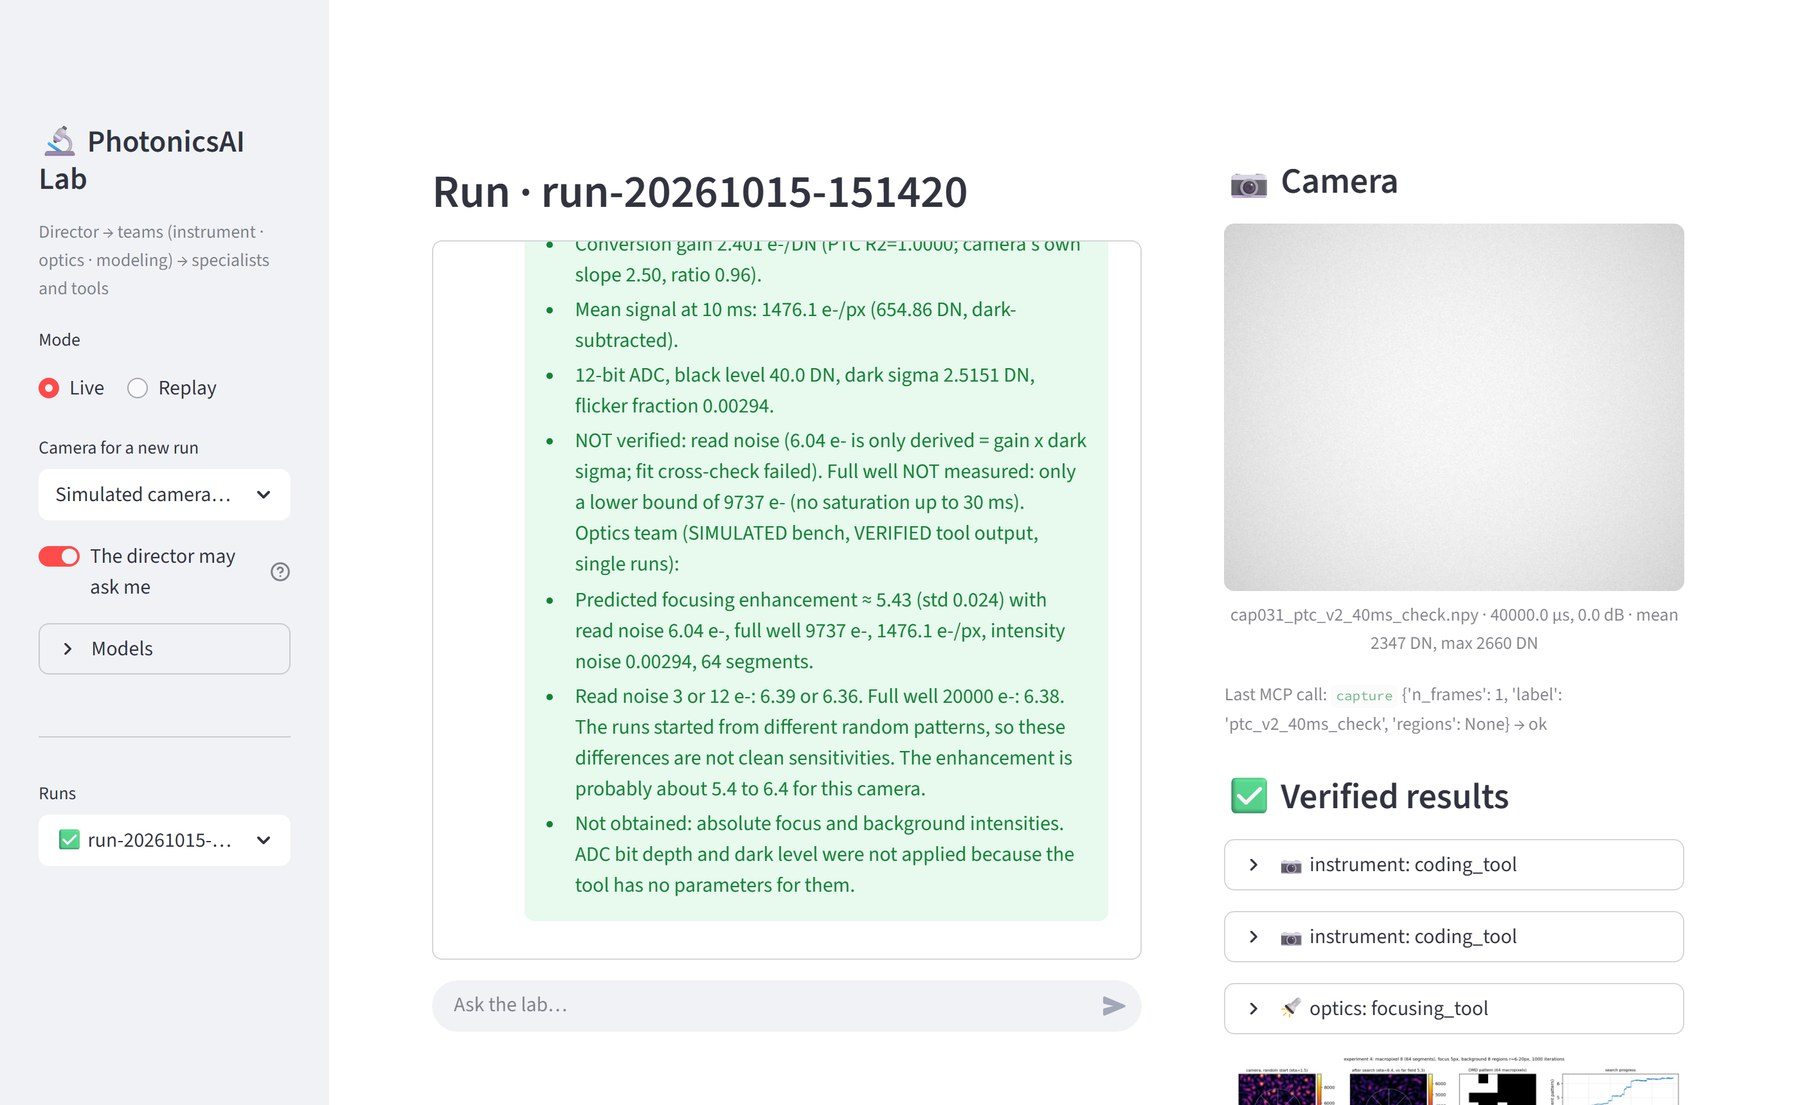
\includegraphics[width=0.8\linewidth,trim={340 0 0 60},clip]{img/ui_run_finished.jpg}\\[4pt]
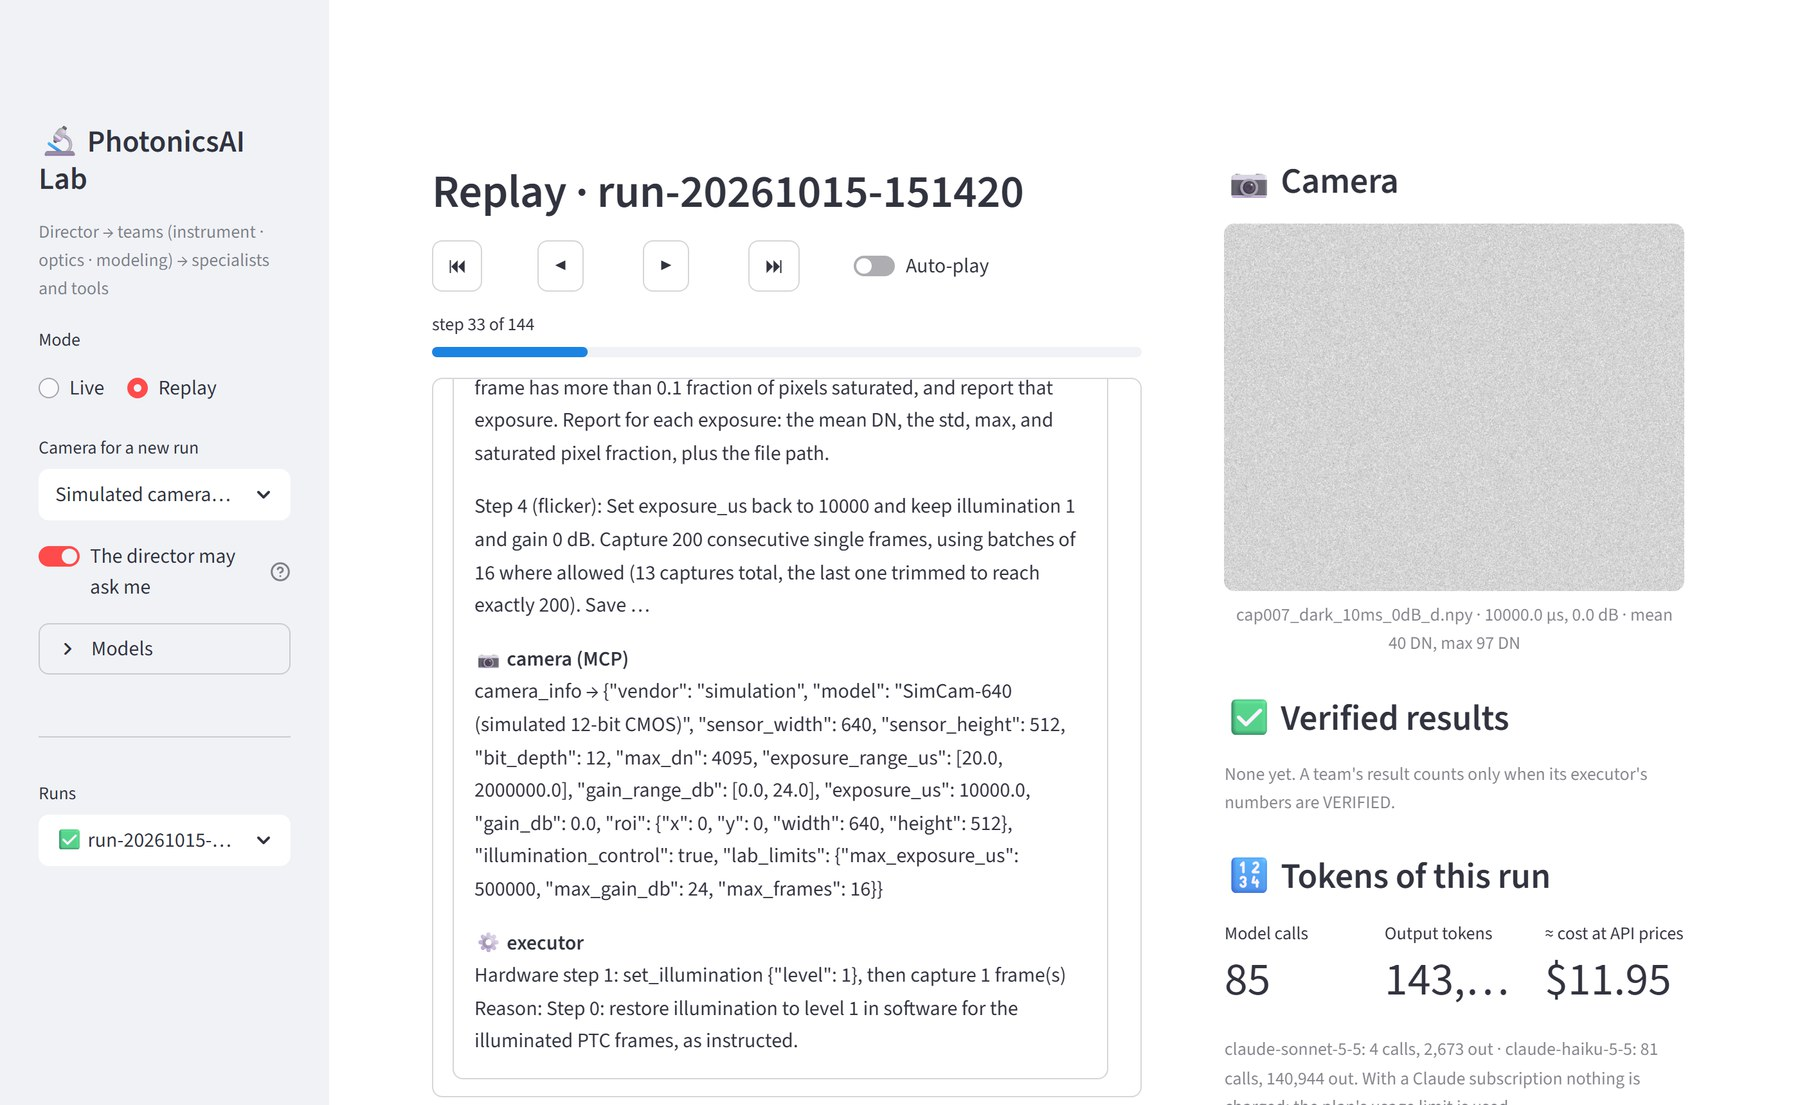
\includegraphics[width=0.8\linewidth,trim={340 0 0 60},clip]{img/ui_replay_team.jpg}
\caption{The app (side bar cut off). Top: the run of section~4 after it finished: the director's final report, the last
camera frame with its settings and the last MCP call, the teams' VERIFIED records. Bottom: the replay of the same run at
step 33, inside the instrument team's work (the executor's hardware steps and the camera's answers through MCP), with
the dark frame captured at that step.}
\end{figure}
\begin{figure}[H]\centering
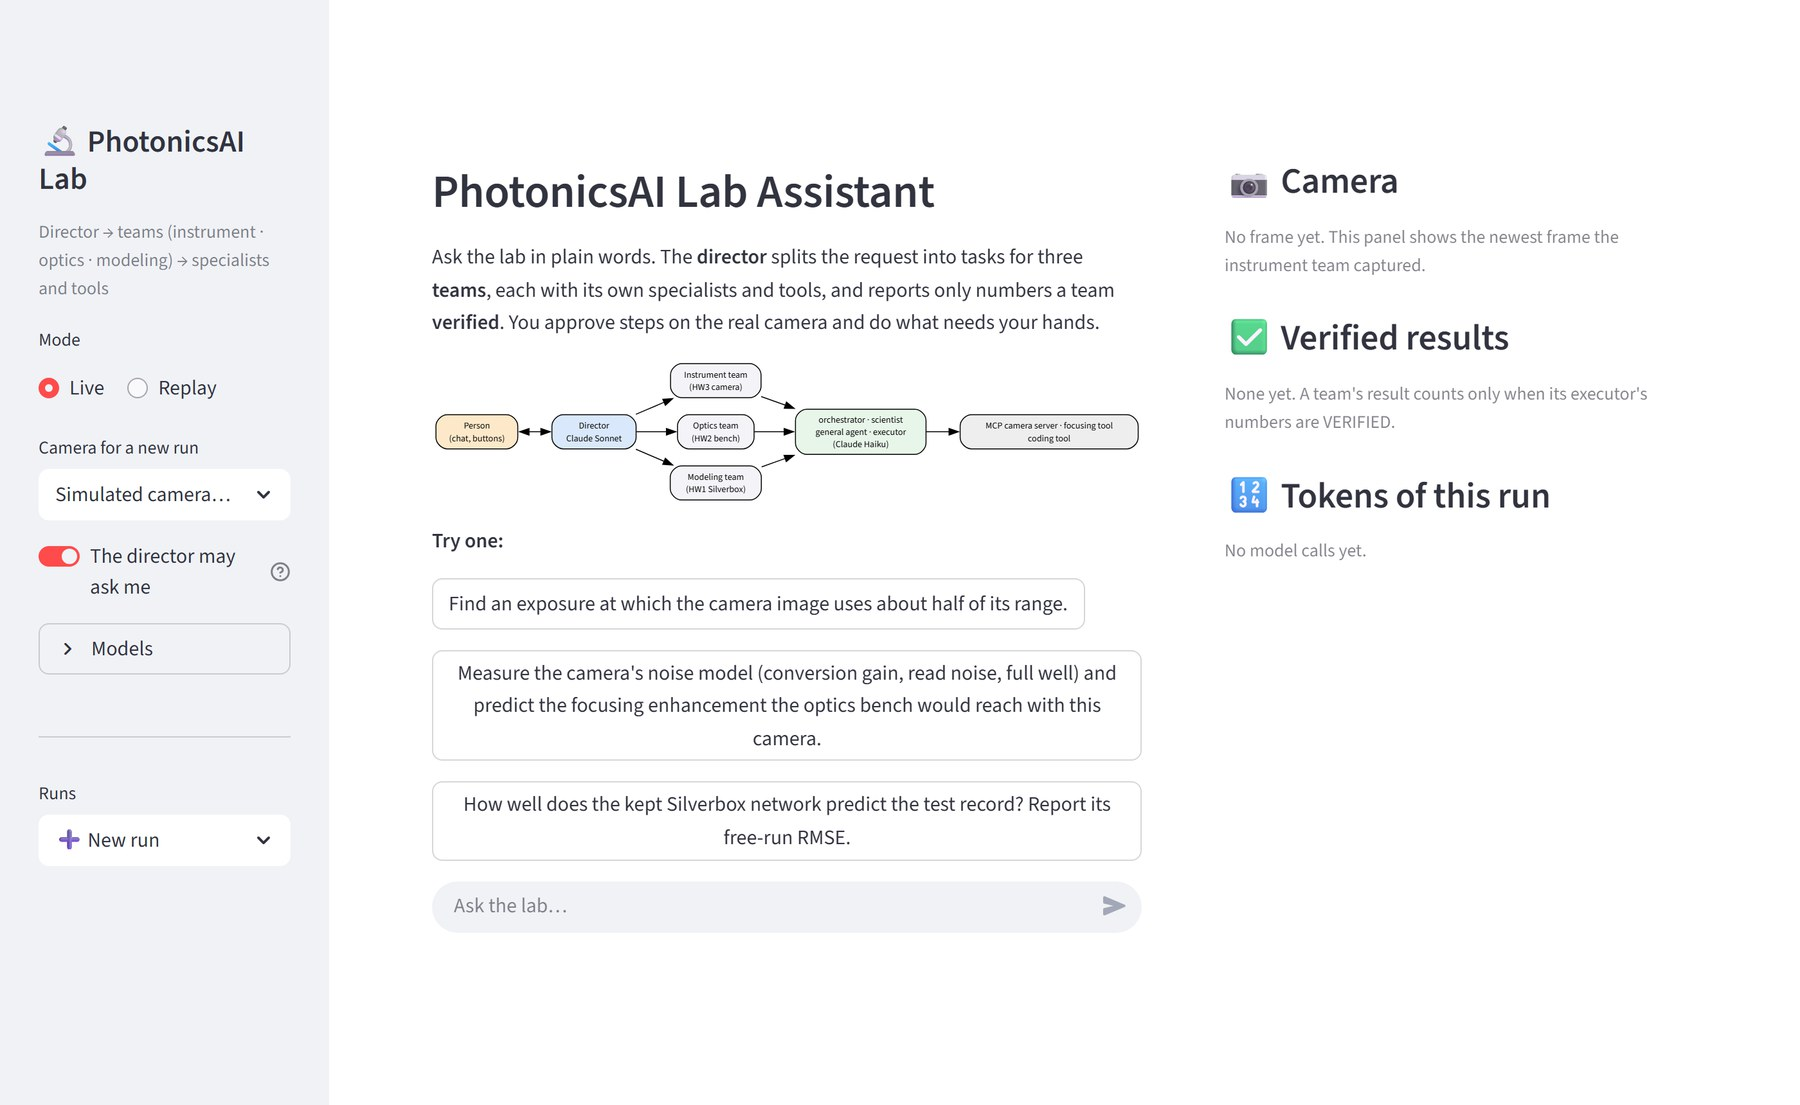
\includegraphics[width=0.495\linewidth]{img/ui_start.jpg}\hfill
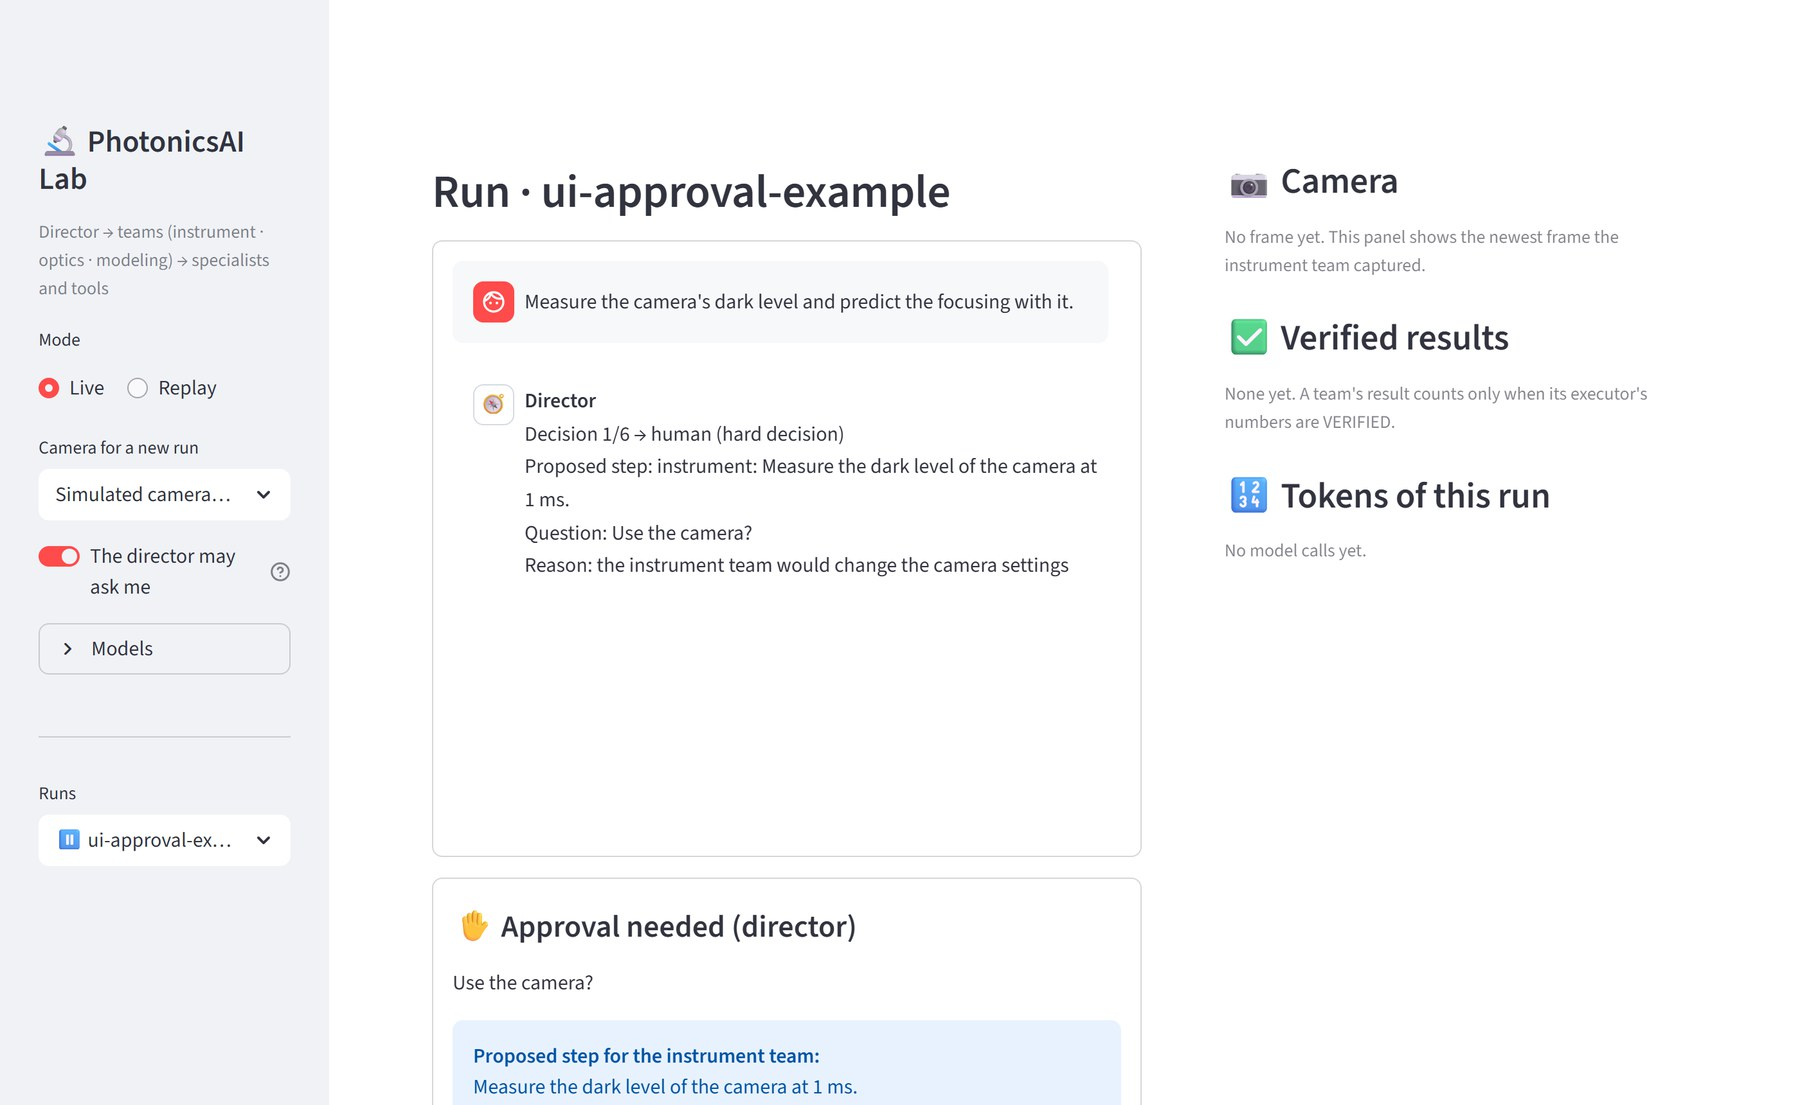
\includegraphics[width=0.495\linewidth]{img/ui_approval.jpg}
\caption{Left: the start page with the hierarchy and three example requests. Right: an approval card (here from an
offline test run with scripted models): the proposed step for the instrument team, Approve and Refuse.}
\end{figure}

%======================================================================
\section*{4. Runs}
%======================================================================
The two camera runs used the simulated camera behind the same MCP server as the real one; the director ran on Claude Sonnet~5.5
and the teams on Claude Haiku~5.5, both with low effort. The runs are in \texttt{lab/runs/} (transcript, events, token
usage, the teams' folders with \texttt{calls.jsonl}, frames, scripts and figures).

\begin{center}\small
\begin{tabularx}{\linewidth}{@{}lXcc@{}}
\toprule
run & request and result & model calls & output tokens\\ \midrule
\texttt{first} & \emph{Find an exposure at which the camera image uses about half of its range.} Instrument team:
  34\,200\,$\mu$s at 0\,dB, mean 2012\,DN = 49.1\,\% of 4095, no saturated pixel, checked by an analysis script on 5
  frames; the exposure set back to its first value afterwards. & 24 (5 + 19) & 32\,971\\
\texttt{run-20261015-151420} & \emph{Measure the camera's noise model and predict the focusing enhancement the optics
  bench would reach with this camera.} Instrument team (two tasks): conversion gain 2.401\,e$^-$/DN (true 2.40), dark
  noise 2.52\,DN, full well $\ge$ 9737\,e$^-$ (true 10\,000), read noise 6.04\,e$^-$ (true 6.0) marked \emph{not verified}
  by the team; optics team with this camera model: enhancement 5.4--6.4 at 64 segments. 14.5 minutes. & 85 (4 + 81) &
  143\,617\\
\texttt{modeling-check} & \emph{How well does the kept Silverbox network predict the test record? Report its free-run
  RMSE.} (director without stops) Modeling team: free-run RMSE 0.422\,mV on the 1024 test samples, 0.70\,\% of the
  test output's standard deviation, equal to the value the metric itself returns (Homework~1: 0.422\,mV); nothing
  retrained. & 18 (2 + 16) & 28\,508\\
\bottomrule
\end{tabularx}
\end{center}

In the second run the instrument team set the ADC to 12 bits and the black level itself before measuring, switched the
light off with \texttt{set\_illumination} for 50 dark frames, and ran a photon-transfer series analysed by its own
scripts. Its first request to the person (``cover the lens'') was answered in words through the action card (``this is
the simulated camera: switch its light off with set\_illumination 0''); the director's prompt now says this itself. The
final report keeps measured and derived numbers apart, names the team for each and states that everything was
simulated. The CLI estimated \$11.95 at API prices; with the subscription nothing is charged, and the plan's usage meter
rose by about 1\,\% of the weekly limit.

The modeling run is the second try of that request. In the first, the team searched for the data file, re-implemented
the metric and finally reported no RMSE, partly because the model sometimes tried to call the coding tool directly
instead of listing it in its structured output. The modeling executor now gets the five lines that evaluate a saved
model, and the CLI backend answers such a slip with a reminder of the protocol and lets the model try again; the
second try returned the verified 0.422\,mV in 18 calls.

\begin{figure}[H]\centering
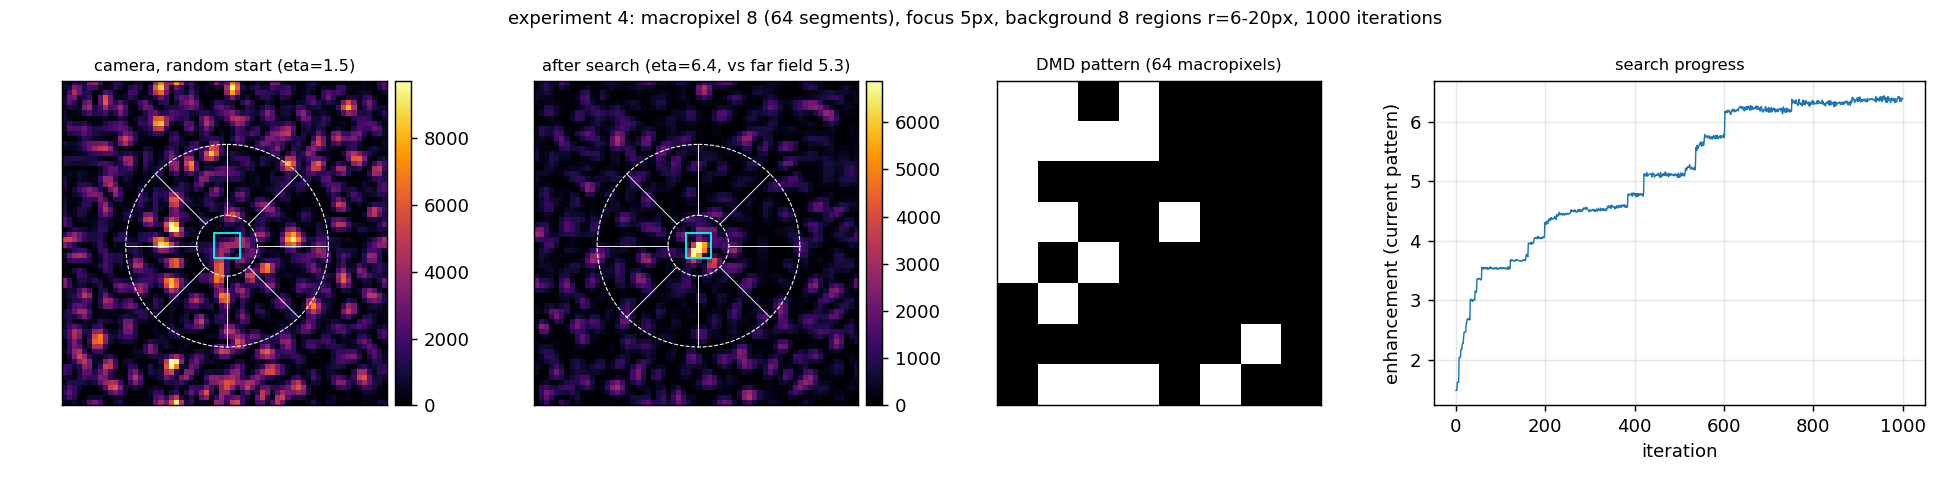
\includegraphics[width=0.9\linewidth]{img/optics_experiment_04.png}
\caption{The optics team's last experiment in that run (simulated HW2 bench with the measured camera model): speckle at
the random start, the focus after 1000 iterations (enhancement 6.4, far field 5.3), the DMD pattern of 64 segments, and
the search progress.}
\end{figure}

%======================================================================
\section*{5. Hardware and the live demonstration}
%======================================================================
The instrument team is the Homework~3 system: the camera's MCP server with 13 tools, the Hikrobot connector through the
MVS SDK, the hardware turn, and the lab limits (500\,ms exposure, 24\,dB gain, 16 frames per capture). On the real camera
the director asks the person once before the instrument team changes its settings, and the team asks the person
whenever a measurement needs hands (blocking and unblocking the light). The live demonstration on 18 October runs the
app with the lab camera (\emph{REAL camera} in the side bar): a short request, the approval card, the camera commands
through MCP and the frames in the camera panel; the longer run of section~4 is shown in the replay mode.

%======================================================================
\section*{6. Tests}
%======================================================================
Without model calls or a camera (scripted models, the real MCP server on the simulated camera):
\begin{itemize}[leftmargin=*,itemsep=1pt]
\item \texttt{lab/tests/test\_lab\_offline.py}: the director's approval; an instrument hardware turn whose question
  (``block the light'') is passed up and answered at the director; a restart of the process between two answers; the
  optics team with the measured camera model; the final report with both VERIFIED records.
\item \texttt{lab/tests/test\_app\_offline.py}: the app's worker thread through the same flow (started while the run is
  still loading, as the page does); the page itself with Streamlit's \texttt{AppTest}: the start page, a finished run,
  the replay controls, and a paused run continued in the page with its approval card.
\item \texttt{cd hw3 \&\& python hw3.py test}: the simulated camera, the MCP server with the new tools, the agent graph.
\end{itemize}

%======================================================================
\section*{7. The token budget}
%======================================================================
The Claude subscription has a 5-hour and a weekly usage limit, shared with every other use, so the design keeps a run
small: Haiku for the teams (81 of the 85 calls of the long run), low thinking effort (36\,\% fewer output tokens per
call in a test), short prompts and reports, a decision budget per level, and at most one approval stop. The meter in
\texttt{claude\_cli.py} adds up every call of the process; each run keeps its own share, also across processes, in
\texttt{transcript.json}, and the app shows it.

%======================================================================
\section*{8. Limits and next steps}
%======================================================================
The lab has no laser for this project, so the optics team's focusing runs on the simulated bench with a camera model
measured on the real camera; the next step is the lab's DMD in front of the camera, as a fourth team or as a tool of the
optics team, so that the HW2 search runs on hardware. No small language model was fine-tuned; the backend already takes
any LangChain chat model, so a local model could take over a team. The director's tasks and the teams' analysis scripts
come from language models and can be wrong; the system therefore reports only numbers that tools printed, keeps the
derived ones apart, and logs every camera command.

\textbf{Run it} (Python 3.11--3.13): \texttt{python -m venv .venv}, \texttt{.venv\textbackslash Scripts\textbackslash
python.exe -m pip install -r requirements.txt}, the Claude Code CLI logged in, and for the real camera Hikrobot MVS with
the camera on USB~3 (MVS client closed). Then \texttt{python -m streamlit run lab/app.py}, or in the terminal
\texttt{python lab/run\_lab.py -{}-thread t1 -{}-camera hikrobot -{}-request "..."}.
\end{document}
